\documentclass[12pt]{article}
\usepackage{fancyhdr}
\usepackage{geometry}
\usepackage{booktabs}
\usepackage{graphicx}
\usepackage{caption}
\usepackage{hyperref}
\usepackage{listings}
\usepackage{xcolor}
\usepackage{amsmath}
\usepackage{amssymb}


\lstdefinestyle{matlab}{
    language=Matlab,
    basicstyle=\ttfamily,
    numbers=left,
    numberstyle=\tiny,
    frame=single,
    backgroundcolor=\color{backcolour},
    commentstyle=\color{codegreen},
    keywordstyle=\color{blue},
    stringstyle=\color{magenta},
    breaklines=true,
}


\definecolor{backcolour}{rgb}{0.95,0.95,0.92}
\definecolor{codegreen}{rgb}{0,0.6,0}
\definecolor{blue}{rgb}{0,0,1}
\definecolor{magenta}{rgb}{1,0,1}


\lstset{style=matlab}

\setlength{\headheight}{14.49998pt}
\addtolength{\topmargin}{-2.49998pt}

\pagestyle{fancy}
\fancyhf{}
\fancyhead[L]{Problem A}
\fancyhead[C]{The University Physics Competition, Team 364}
\fancyhead[R]{\thepage} 
\fancyheadoffset[R]{0.4cm}

\renewcommand{\headrulewidth}{1pt}

\geometry{top=2.5cm,bottom=2.0cm,left=2.8cm,right=2.0cm}

\title{Space Diving}
\author{Team 364, Problem A}

\begin{document}

\maketitle 
\thispagestyle{fancy}

\begin{abstract}

This paper is based on the theme of high-altitude skydiving by an individual wearing a spacesuit. We begin by making reasonable assumptions 
and proceed to analyze the various motion states and influencing factors throughout the skydiving process. We establish motion equations, 
compute maximum values, and simplify the entire skydiving procedure into two distinct stages: pre-parachute deployment and post-parachute 
deployment. We also examine the associated force conditions, take into account the variation of atmospheric density with altitude, and 
establish motion equations to calculate a maximum skydiving altitude of 57,800 meters, without factoring in the parachute deployment.
\textbf{Subsequently}, we delve into an analysis of the parachute deployment process, highlighting the significant impact of the critical 
opening speed of the parachute and the opening load on jump height and the overall procedure. Through a detailed examination of the critical
opening speed of the parachute and the optimization of equations, we further constrain the maximum attainable altitude. It is 
determined that the highest achievable skydiving altitude, while ensuring the safety of the entire skydiving process, is 44,110 meters.
\textbf{Furthermore}, our research considers the maximum acceleration tolerable for the human body and the opening load 
to guarantee the individual's safety throughout the skydiving experience. In conclusion, we establish that the maximum safe 
skydiving altitude achievable is 44,110 meters.

\end{abstract}

\newpage 
\tableofcontents

\newpage

\section{Problem restatement}

Suppose there is a situation where a rocket carries a skydiver vertically to a substantial altitude, 
potentially above Earth's atmosphere. Upon reaching this height, the skydiver jumps from the rocket while wearing a space 
suit and parachute, initiating the descent back to Earth's surface. Assess the challenges and risks 
involved in this descent, given that the total mass of the skydiver, space suit, and parachute is 190 kg. Calculate the 
maximum altitude from which a person could safely make the descent to reach the Earth's surface.

\section{Assumptions}

\begin{enumerate}
    \item The parachute deployment location always remains at the equator.
    \item Due to the location at the equator, horizontal wind speeds in various atmospheric layers are generally low. 
    Therefore, in the following model, the influence of crosswinds on parachute descent will not be considered.
    \item In the majority of cases, at the moment when a parachutist 
    jumps from the rocket, the rocket does not possess any relative 
    vertical velocity over the Earth's surface.
\end{enumerate}

\section{Nomenclature of constants}
Symbols that are not annotated will be explained within the text.

\begin{table}[h]
    \centering
    \begin{tabular}{c c c}
    \toprule
    Symbol & definition \\
    \midrule
    $c_h$ & drag coefficient of Human  & 0.47 \\
    $c_p$ & drag coefficient of Parachute & 0.8 \\
    $g$ & gravitational acceleration & $9.80665 \text{m/s}^2$\\
    $G$ & gravitational constant & $6.67430\times 10^{-11} \text{N}\cdot\text{m}^2\cdot\text{kg}^{-2}$\\
    $m$ & total mass of Space Diver & $190\text{kg}$\\
    $M$ & Earth mass & $5.972168\times 10^{24} \text{kg}$\\
    $M_a$ & molar mass of Earth's air & $0.0289644 \text{kg/mol}$ \\
    $r_0$ & Earth radius & 6371.0 km \\
    $R^*$ & universal gas constant & $8.3144598 \text{N}\cdot\text{m/(mol·K)}$ \\
    \bottomrule
    \end{tabular}
\end{table}

\section{Two primitive models}

\subsection{The Simplest model}

\subsubsection{Model establishment}

Given that the complexity of this problem, 
we first consider an extremely simplified model.  
Assume that throughout the entire process, gravitational acceleration remains constant, air density 
remains constant, the air drag coefficient remains constant, and the parachutist 
remains within an atmospheric environment with a density equivalent to that near the
Earth's surface. The parachutist begins the descent from an initial state with zero 
relative ground velocity. 

Hence, we divide this process into the following two phases:

\begin{itemize}
    \item \textbf{Phase One:} From the moment the person jumps from the rocket until the parachute is deployed.
    \item \textbf{Phase Two:} From parachute deployment to a safe landing.
\end{itemize}

In Phase One, the person begins to descend with an initial velocity of zero and experiences vertical downward gravitational force along with vertical upward air resistance. 
The net external force is the gravitational force minus the air resistance, resulting in downward acceleration. The person undergoes vertical downward acceleration.

Therefore, according to the drag equation\cite{enwiki:1144175318}, derive the motion equations for the descent process before the parachute is deployed: 

\[ \ddot{r} = - GM\frac{1}{r^2} + \frac{1}{2}\frac{c_h\rho A_h}{m}\dot{r}^2\]

Where: 
\begin{itemize}
    \item $r$ refers to the distance between the parachutist and the center of earth. 
    \item $A_h$ refers to the reference area of a human when falling straight down.
\end{itemize}

In Phase Two, the person deploys the parachute. Neglecting the time it takes 
to deploy the parachute and its effect on the person's motion, the person's 
velocity remains constant.

At this point, considering the parachute and the person as a single entity, 
a force analysis can be conducted on them.

Hence, we can continue using the above formula, with the only modification being to replace the drag coefficient 
and reference area with coefficients associated with the parachute.

So in this case, 
\[ \ddot{r} = - GM\frac{1}{r^2} + \frac{1}{2}\frac{c_p\rho A_p}{m}\dot{r}^2\]
where $A_p$ refers to the reference area of the parachute.

Consider the human as a cylindrical object. The reference area of a person when falling straight down with a prone position 
is about one square meter, 
and the drag coefficient would be around 0.47\cite{enwiki:1160706380}.

For a medium-sized parachute, the effective area is approximately 70 square meters. 
In the case of high-speed descent parachutes (such as when initially deploying the parachute and 
descending rapidly), the drag coefficient may be in the range of 0.8 to 1.2. 
For low-speed descent parachutes (such as when slowing down during the descent), 
it may be in the range of 1.2 to 1.5.

\subsubsection{Calculation}
For example, when a person begins to descend from a height of 50 kilometers above the ground, without deploying the parachute, 
the variation of their velocity and height respect to time is depicted in the following figure:

\begin{figure}[!hbtp]
    \centering
    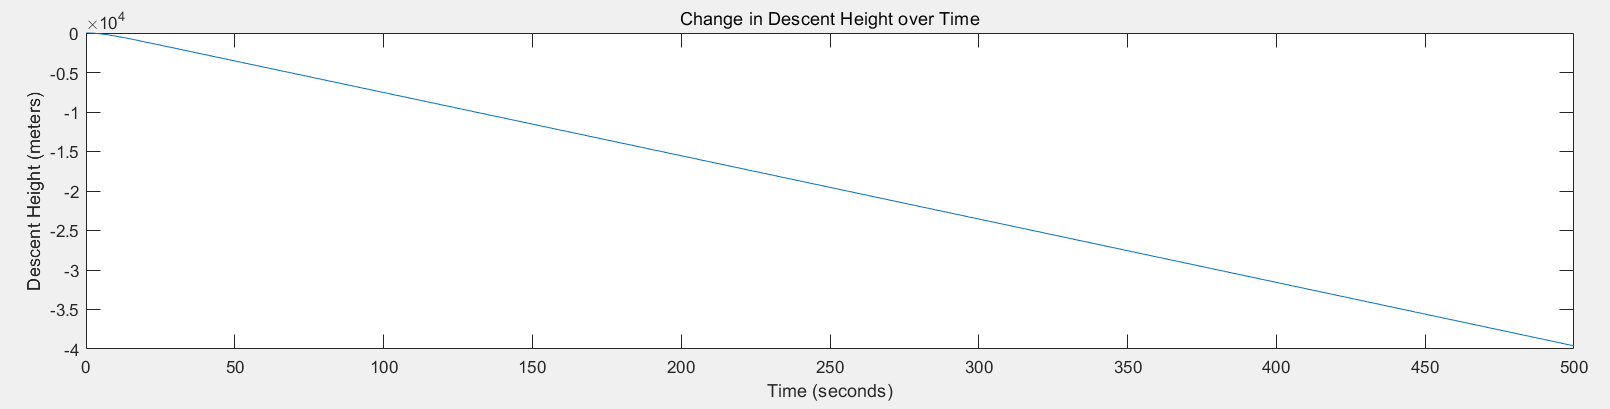
\includegraphics[width = 0.7\linewidth]{image/001.png}
    \caption{Height change over time before parachute}
\end{figure}
\begin{figure}[!hbtp]
    \centering
    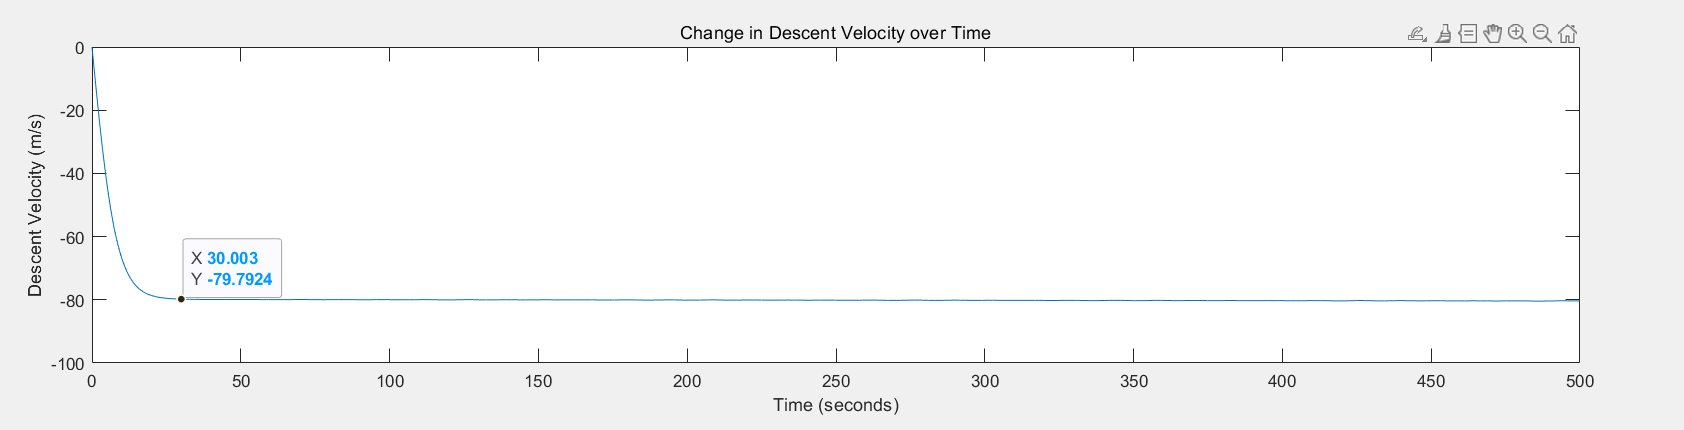
\includegraphics[width = 0.7\linewidth]{image/002.png}
    \caption{Velocity change over time before parachute}
\end{figure}

From this, we can observe that the velocity of the parachutist will roughly stabilize at 
a constant value within about 30 seconds, followed by a gradual increase. When the height is sufficiently high, 
this velocity can be considered as the initial velocity at the time of parachute deployment.

Similarly, the following charts can be derived:
\begin{figure}[!hbtp]
    \centering
    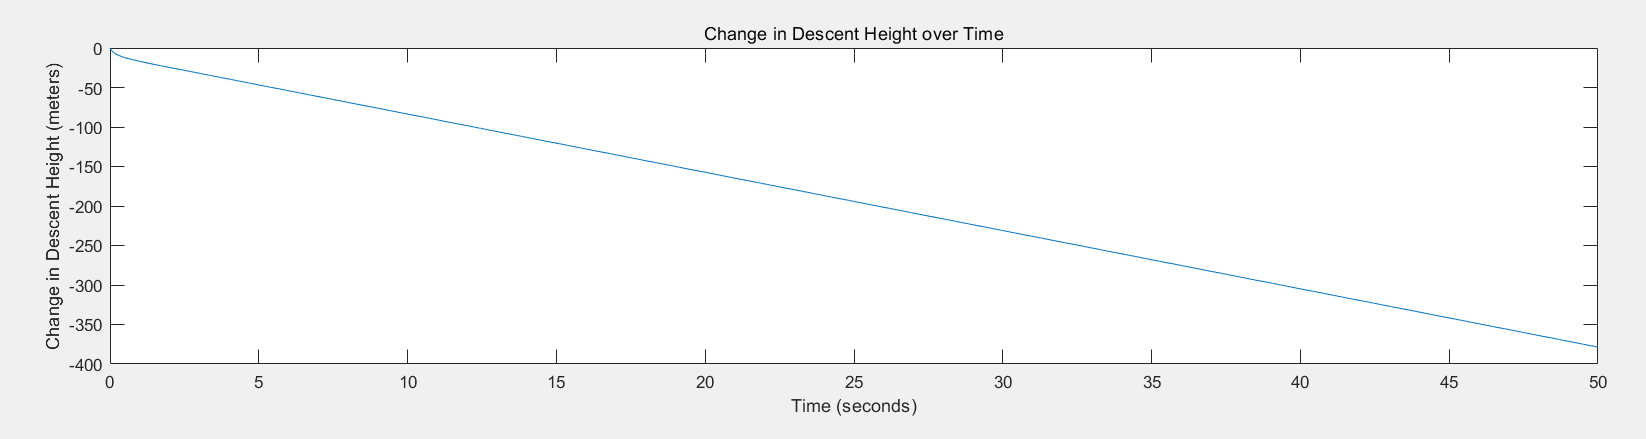
\includegraphics[width = 0.7\linewidth]{image/003.png}
    \caption{Height change over time after parachute}
\end{figure}
\begin{figure}[!hbtp]
    \centering
    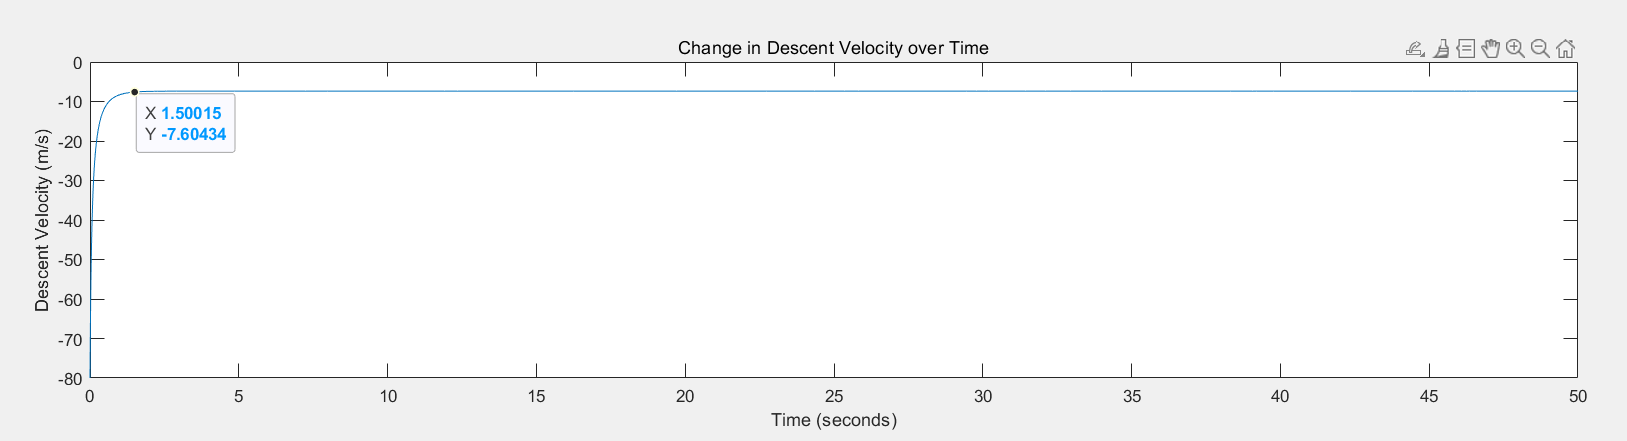
\includegraphics[width = 0.7\linewidth]{image/004.png}
    \caption{Velocity change over time after parachute}
\end{figure}

\begin{minipage}{0.5\linewidth}
    The final landing velocity is approximately 7.6 meters per second, which is within the range of a safe 
    landing speed for a human.

    However, in this scenario, the instantaneous gravitational acceleration 
    at the moment of parachute deployment reaches $1000 m/s^2$, which is unbearable for the human body. 
    Additionally, the parachute lines would also struggle to withstand such immense forces.

\end{minipage}
\hfill
\begin{minipage}{0.4\linewidth}
    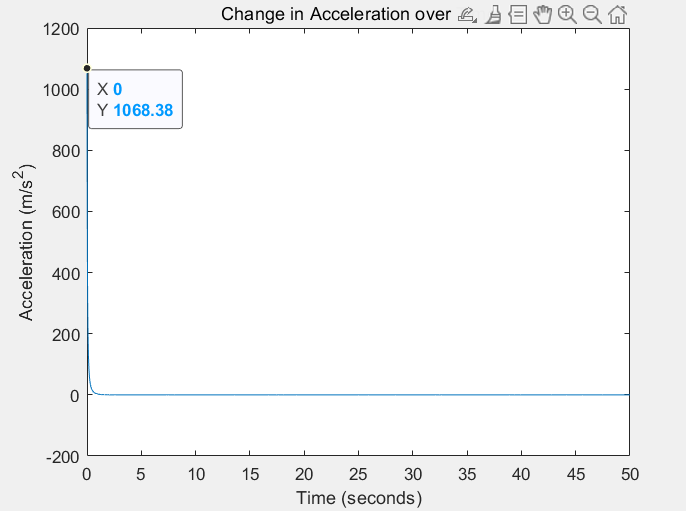
\includegraphics[width = \linewidth]{image/005.png}
    \captionof{figure}{Acceleration change over time after parachute}
\end{minipage}
\vspace{6pt}

And at the same time, Indeed, the density of the Earth's atmosphere varies with altitude in reality. 
In space, it is not possible to have such a dense atmosphere. 
The model needs further optimization to account for these variations.

\subsection{Model taking into account variations in atmospheric density}

\subsubsection{Model establishment}
As is mentioned before, in this subsection, the variations in atmospheric density will be taken into account. 
In general, air pressure and density decrease with altitude in the atmosphere. However, the temperature has a more complicated 
profile with altitude, and may remain relatively constant or even increase with altitude in some regions\cite{enwiki:1181726796}.

When it comes to a space diving, The entire jumping process involves significant changes in altitude. The parachutist not only 
crosses the troposphere but may also pass through the stratosphere, and it's even possible to jump from the mesosphere.


\begin{figure}[!hbtp]
    \centering 
    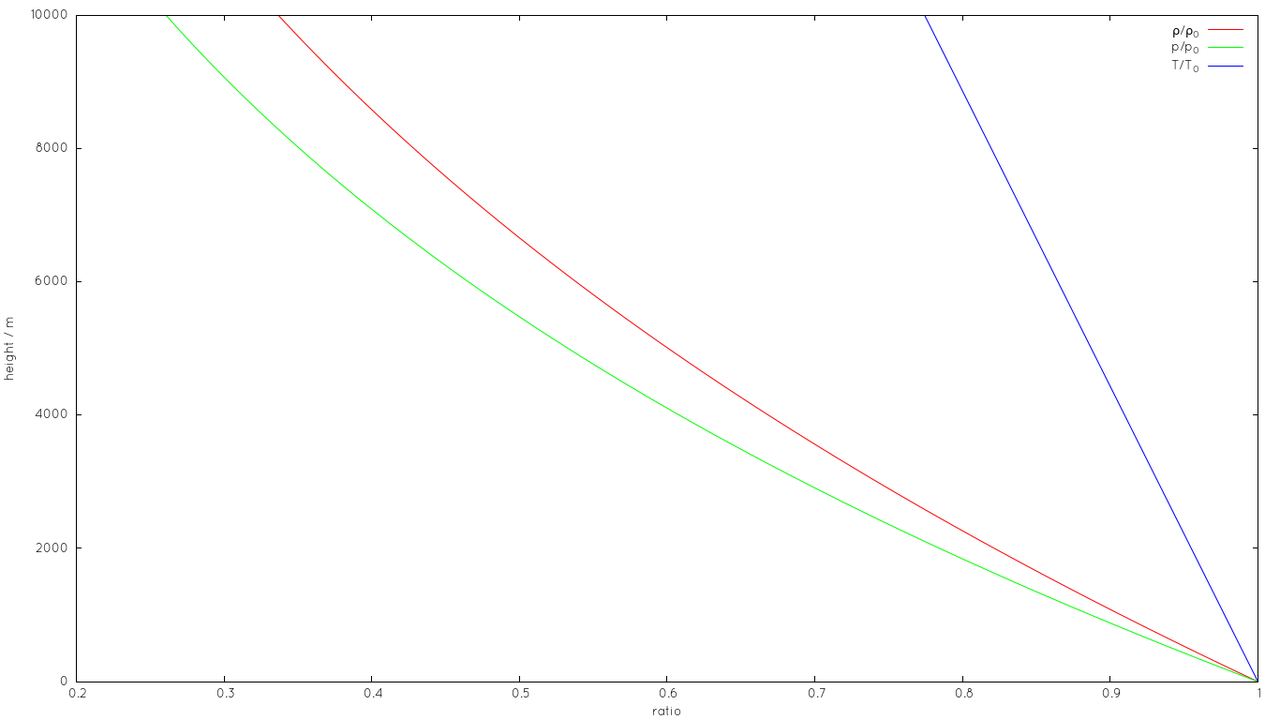
\includegraphics[width = 0.6\linewidth]{image/007.png}
    \caption{Ratio of atmospheric density to standard density ($ 1.225 \text{kg/m}^3$) in troposphere\cite{enwiki:1181726796}}
\end{figure}

The air density equation applicable to the standard model of the troposphere and mesosphere in which the temperature is 
assumed to vary with altitude at a lapse rate of $L_b$ \cite{enwiki:1179305813}:
\[ \rho = \rho_b\left[ \frac{T_b - (h - h_b)L_b}{T_b}\right]^{\left( \frac{gM_a}{R^L_b} - 1\right)}\]

The air density equation applicable to the standard model of the stratosphere 
in which the temperature is assumed not to vary with altitude\cite{enwiki:1179305813}:
\[ \rho =  \rho_b \text{exp}\left[\frac{-gM_a(h - h_b)}{R^*T_b}\right]\]

Where:
\begin{itemize}
    \item $\rho $ = mass density 
    \item $T_{b}$ = standard temperature 
    \item $L$ = standard temperature lapse rate (see table below) 
    \item $h$ = height above sea level
\end{itemize}

To simplify the calculation, $g$ is considered as a constant value.

The value of subscript $b$ ranges from 0 to 6 in accordance with each of seven successive layers 
of the atmosphere shown in the table below. The reference value for $\rho_b$ for $b$ = 0 is the defined 
sea level value. Values of $\rho_b$ of $b$ = 1 through $b$ = 6
are obtained from the application of the appropriate member of the pair equations 
1 and 2 for the case when $h = h_{b+1}$ \cite{usatmosphere1976}.

\begin{figure}[!hbtp]
    \centering 
    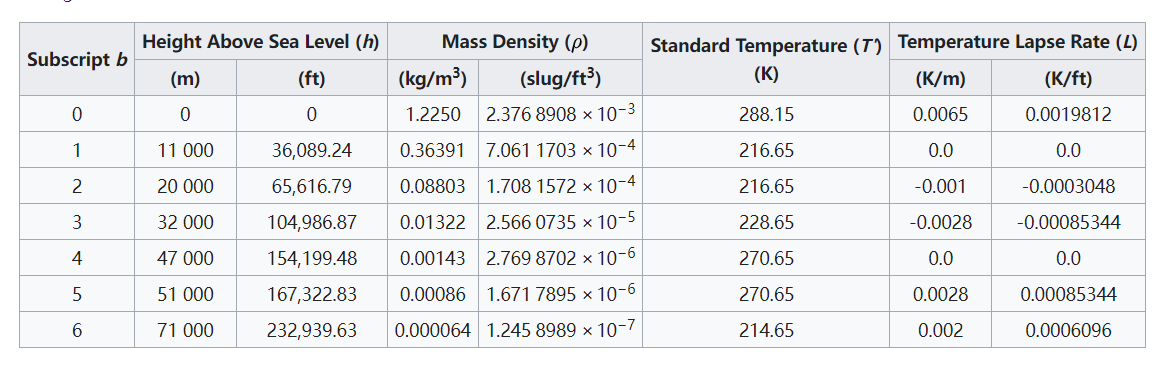
\includegraphics[width = 0.8\linewidth]{image/008.png}
    \caption{Atmospheric data\cite{usatmosphere1976}}
\end{figure}

\subsubsection{Calculation}

\begin{minipage}{0.3\linewidth}
    Based on the observed data table provided earlier, we can calculate the variation in air density 
    for different atmospheric layers. 
\end{minipage}
\hfill
\begin{minipage}{0.7\linewidth}
    \centering 
    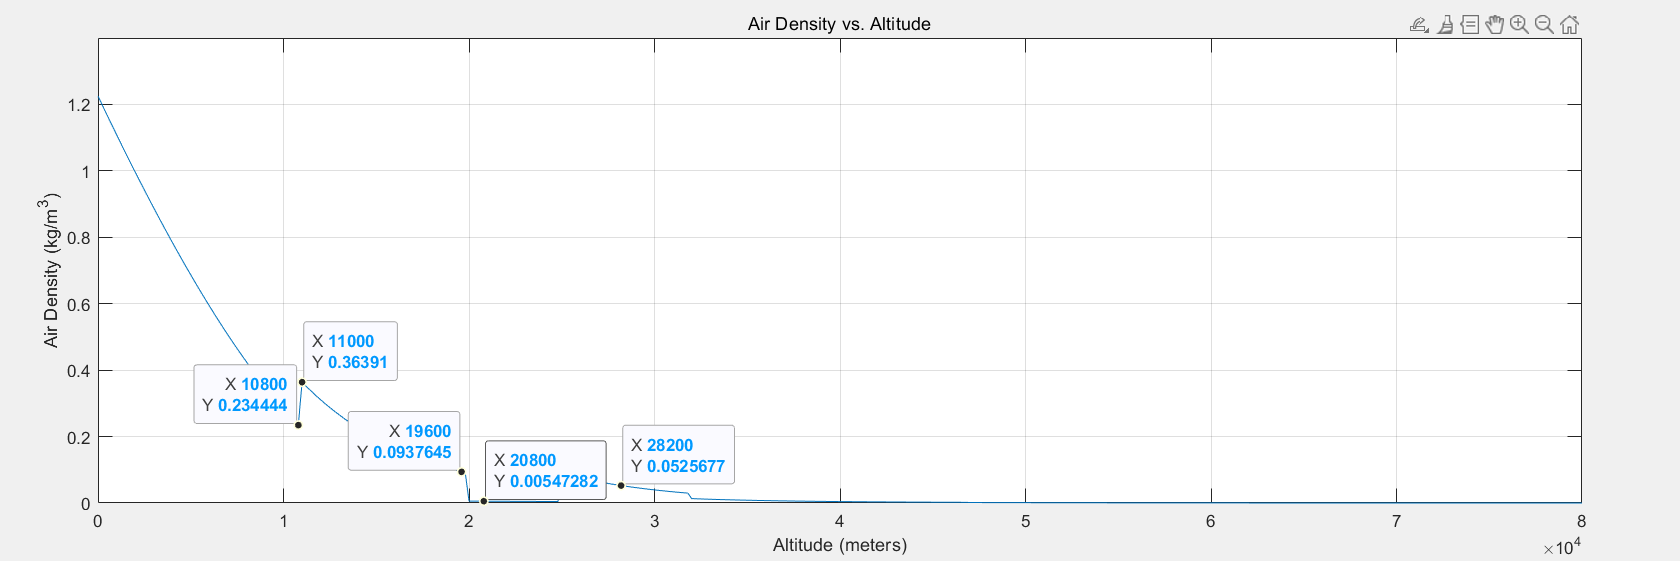
\includegraphics[width = 0.8\linewidth]{image/009.png}
    \captionof{figure}{Air Density vs. Altitude}
\end{minipage}

\vspace{12pt}
Here are the graphical results obtained through MATLAB (The code is included in the appendix.) calculations.

To simplify the calculations, the relationship between air pressure and 
altitude is fitted as an exponential function. The graph is as follows:

\begin{figure}[!hbtp]
    \centering 
    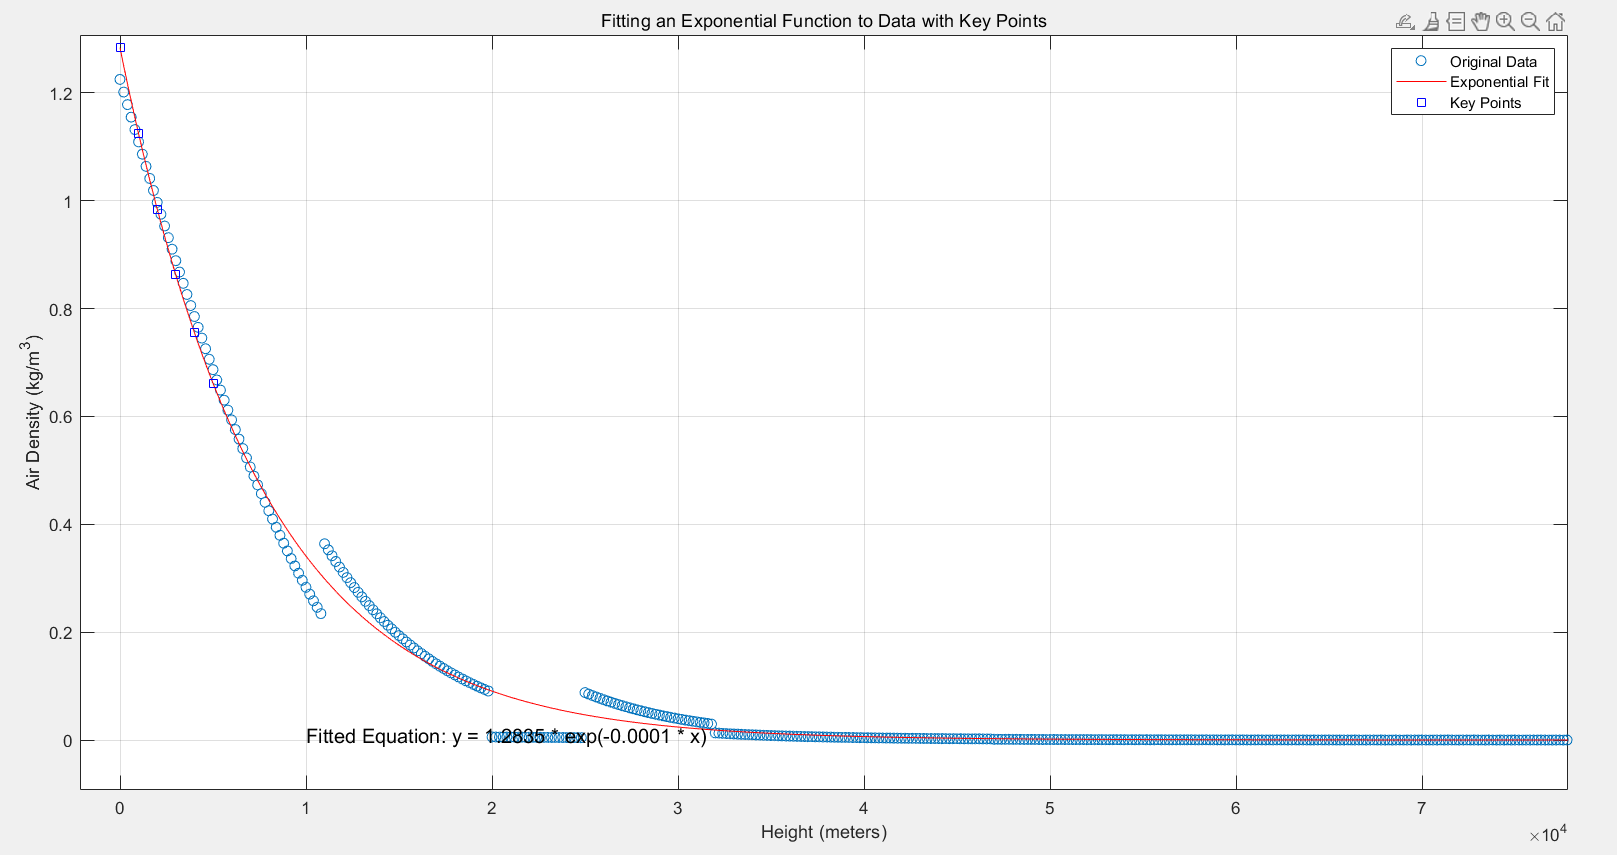
\includegraphics[width = 0.8\linewidth]{image/010.png}
    \caption{Fitted curve}
\end{figure}

From this, we can deduce the relationship between atmospheric density and altitude as follows:
\[ \rho = 1.2835e^{-0.001h}\]

Where $\rho $ is density and $h$ is height above sea level.

Add this to \textit{4.1 model}:

\[ \ddot{r} = - GM\frac{1}{r^2} + \frac{0.64175e^{-0.001(r - r_0)} c_h A_h}{m}\dot{r}^2\]

However, due to the rapid decrease in atmospheric density at higher altitudes during 
the fitting process, we decided to 
use a constant density (\( \rho \)) for the entire process beyond a certain altitude.

Taking the example of a descent from a height of 39 kilometers, we used 
\( \rho = 0.01322 \) to calculate the process during the first 
fifty seconds, which corresponds to the descent of the first ten thousand meters.

\begin{figure}[!hbtp]
    \centering 
    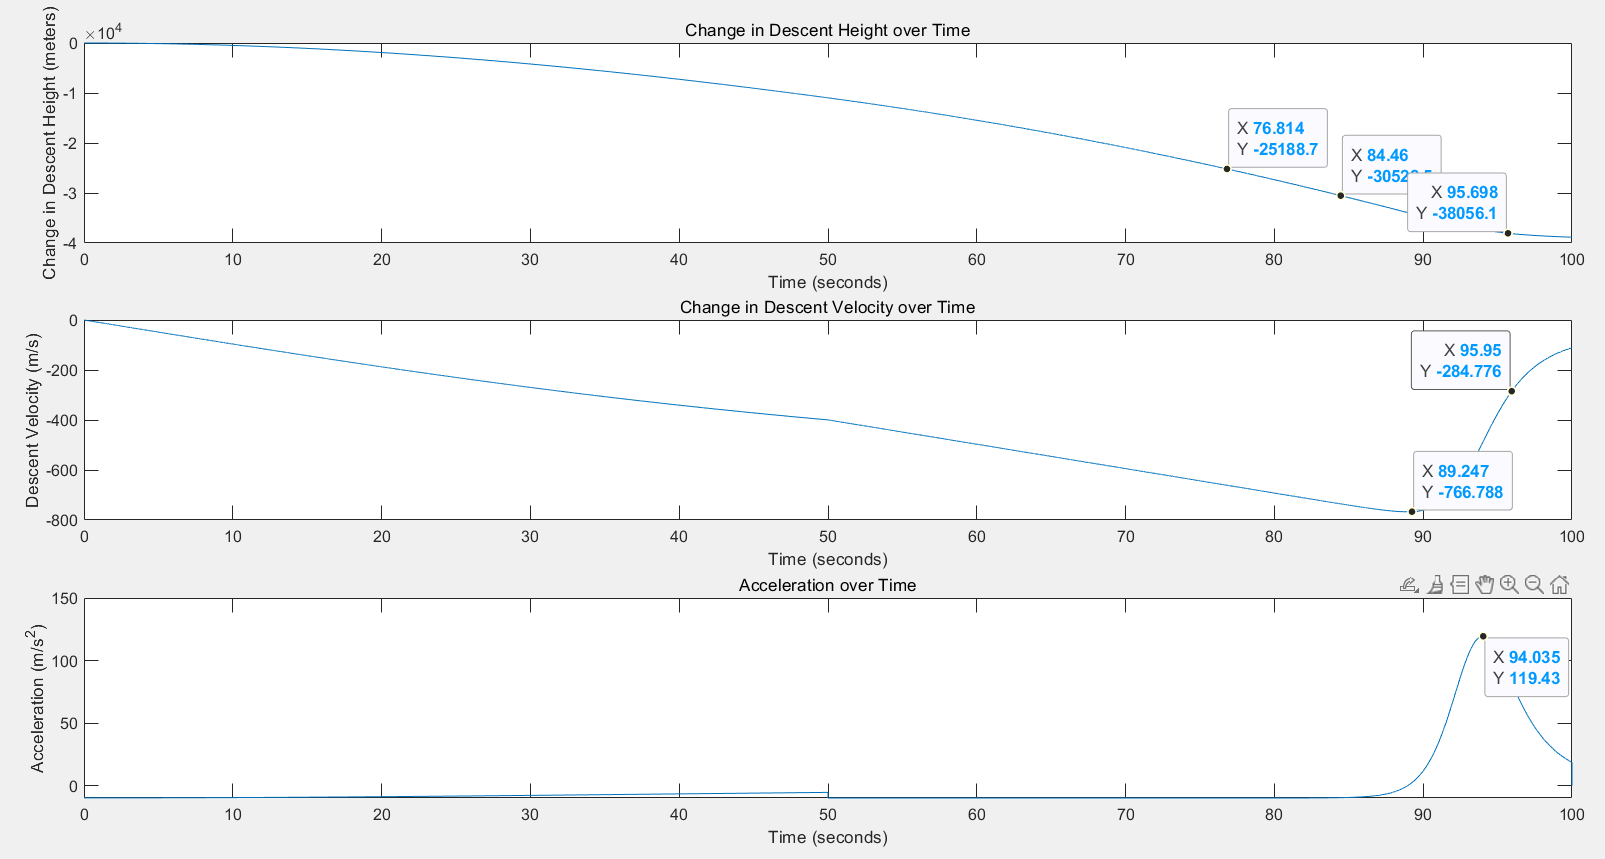
\includegraphics[width = 0.6\linewidth]{image/011.png}
    \caption{Motion graphics}
\end{figure}

From the graphics, we can observe that the maximum acceleration during the entire 
process reaches $119.43 \text{m/s}^2$, and at a distance of approximately 1000 meters above the ground, the descent speed is  
280 meters per second.

Due to the upper limit of G-forces that a human can withstand, 
we need to constrain the maximum acceleration during the process 
to determine the highest possible jumping altitude.

The human tolerance to G-forces in different directions is depicted in the following figure\cite{enwiki:1183575400}:
\begin{figure}[!hbtp]
    \centering 
    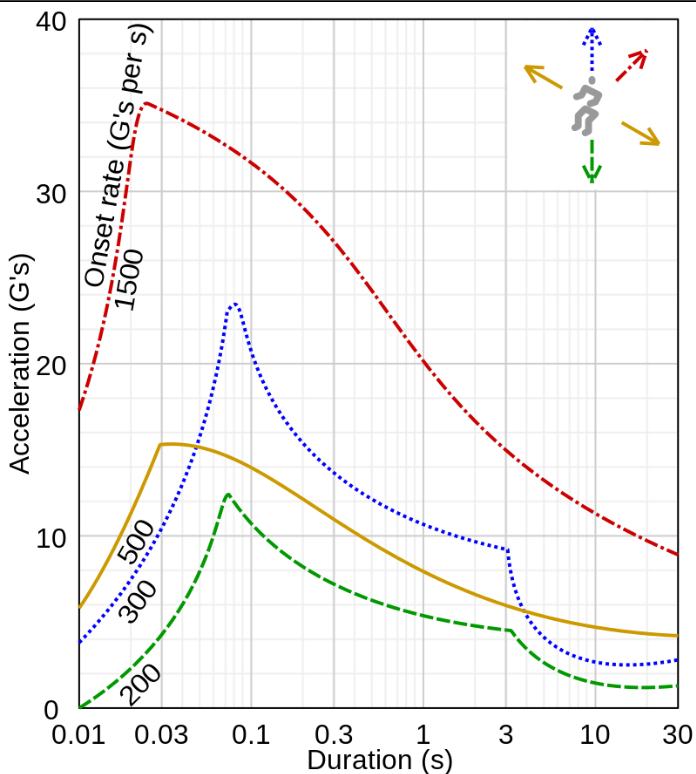
\includegraphics[width = 0.3\linewidth]{image/012.png}
    \caption{Human tolerance}
\end{figure}

Since in our model, the person is descending in a prone position, we can establish the 
following constraints with reference to the red dashed line:

The average acceleration within any one-second interval should be less than 20 Gs.
\[\overline{a}_{t, (t+1)} < 20g\]

And we can see:
\begin{figure}[!hbtp]
    \centering 
    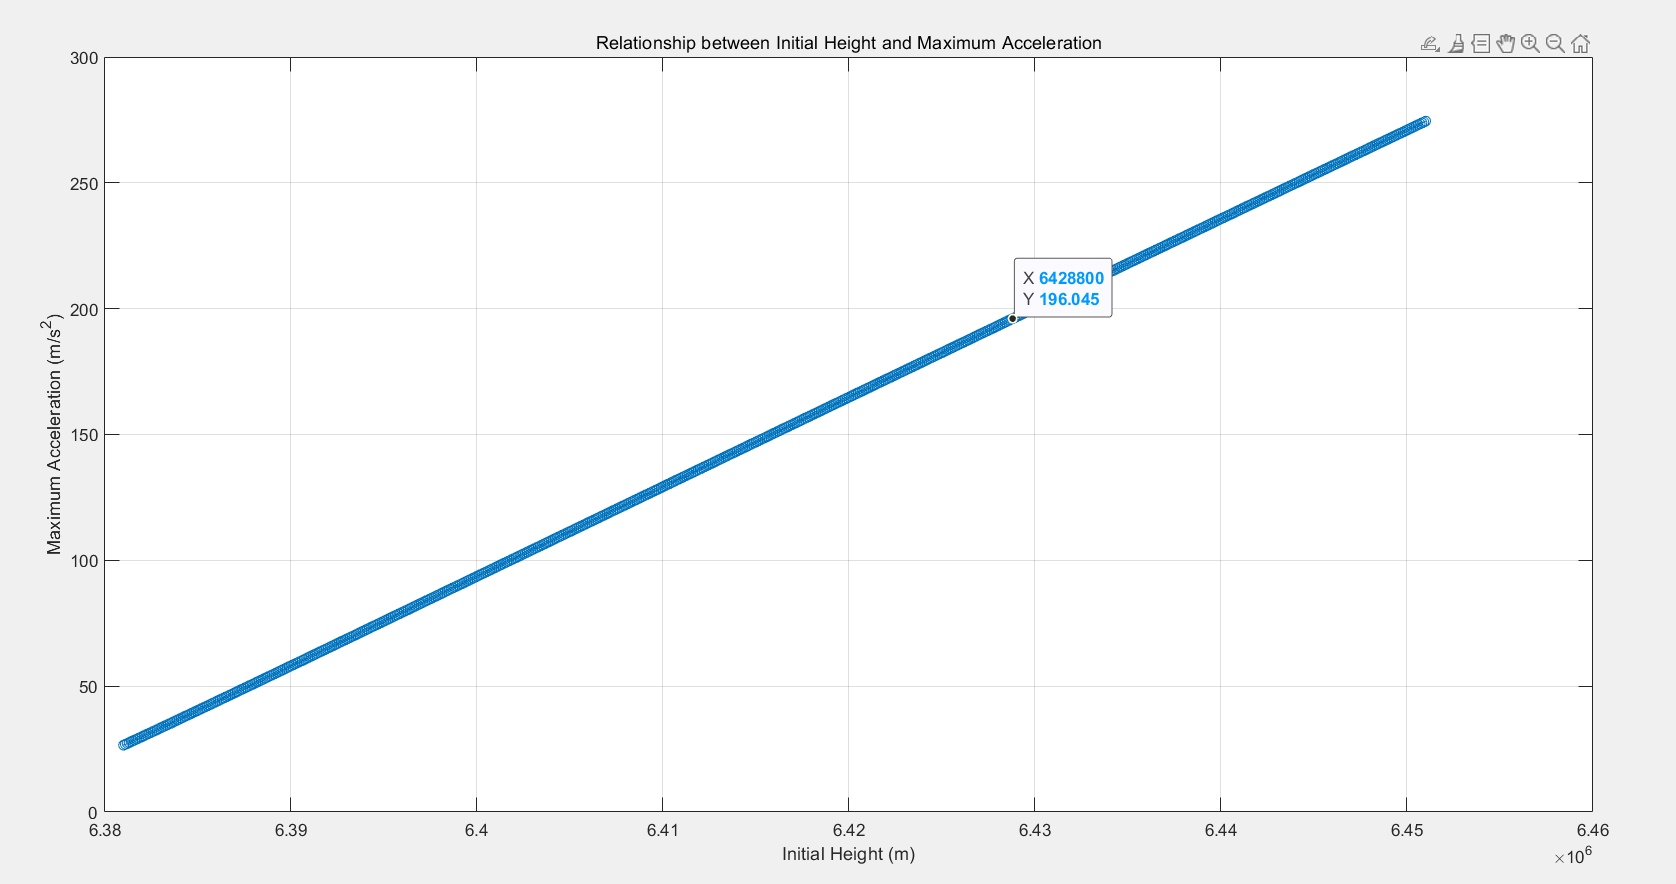
\includegraphics[width = 0.8\linewidth]{image/013.png}
    \caption{Relationship between initial height and maximum acceleration}
\end{figure}

Based on the human tolerance for acceleration, we can determine that the maximum descent 
altitude is approximately \textbf{57,800 meters}.

In this scenario, the motion graphic is as follows:
\begin{figure}[!hbtp]
    \centering 
    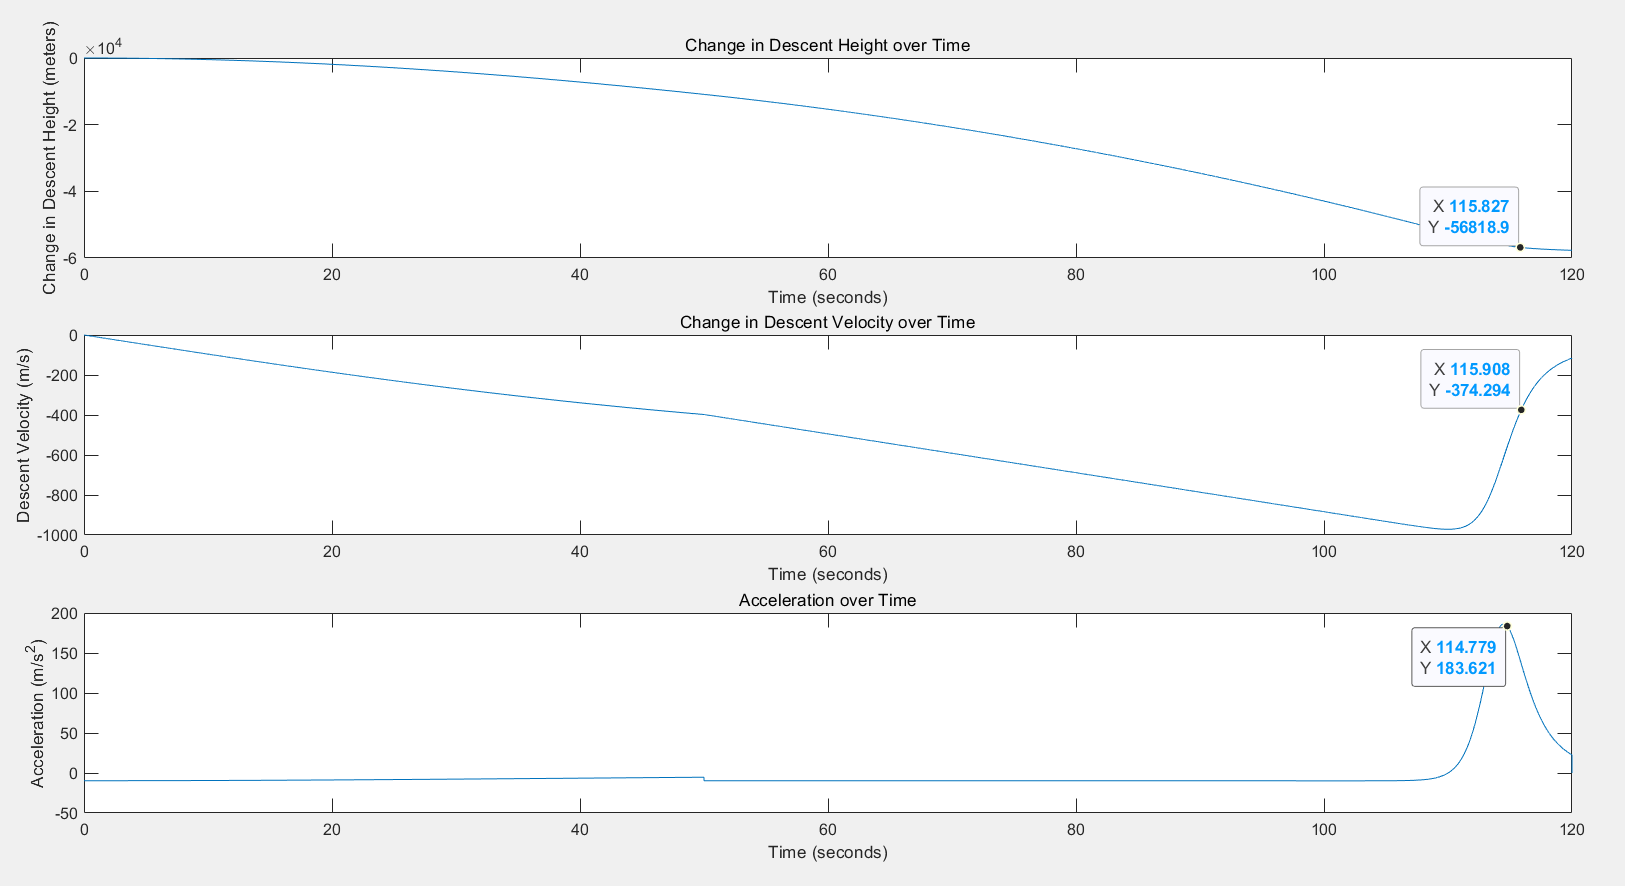
\includegraphics[width = 0.8\linewidth]{image/014.png}
    \caption{Motion graphics}
\end{figure}

Since the atmospheric density remains relatively constant after 
parachute deployment and in alignment with the analysis of the \textit{4.1 model}, 
we only considered the motion process before the parachute is deployed in this section.

\subsubsection{Conclusion}

Our research on acceleration has been successful. However, 
the final result shows that at a height of approximately one kilometer 
above the ground, the person's speed is still around 370 meters per second, 
which is a highly dangerous speed for parachute deployment. At a height of about 
200 meters above the ground, the speed is still 115 meters per second, which is below 
the safe parachute deployment altitude. Therefore, we need to conduct a more detailed 
study of the motion at the moment of parachute deployment, which will be addressed later.

\section{Models with optimized key states}

\subsection{Critical speed for parachute deployment}
During the process of parachute inflation, specific boundary conditions are 
necessary for the parachute to fully inflate. When the opening speed of the parachute 
reaches a certain level, the parachute may reach a "jellyfish" state, where it cannot fully 
inflate, and with increasing speed, the volume of the inflated parachute gradually decreases.

The maximum oncoming flow velocity at which the parachute can fully inflate is defined as 
the critical opening speed. The critical opening speed is dependent on the amount of gas 
entering the parachute and the amount of gas leaving the parachute. When the gas entering 
the parachute is greater than the gas leaving it, the parachute can fully inflate; otherwise, 
the parachute assumes a "jellyfish" state.

To calculate the critical opening speed, we assume the inflation state of the parachute resembles 
a light bulb, and the outer shape of the canopy is approximated as a combination of a hemisphere and 
a frustum, as shown in the figure. The conditions for the expansion of the parachute during inflation 
occur when the volume of gas entering the canopy is greater than the volume of gas exiting the canopy. 
Assuming incompressible flow conditions and neglecting changes in gas density, the variation in the internal 
volume of the canopy can be expressed as:

\begin{figure}[!hbtp]
    \centering 
    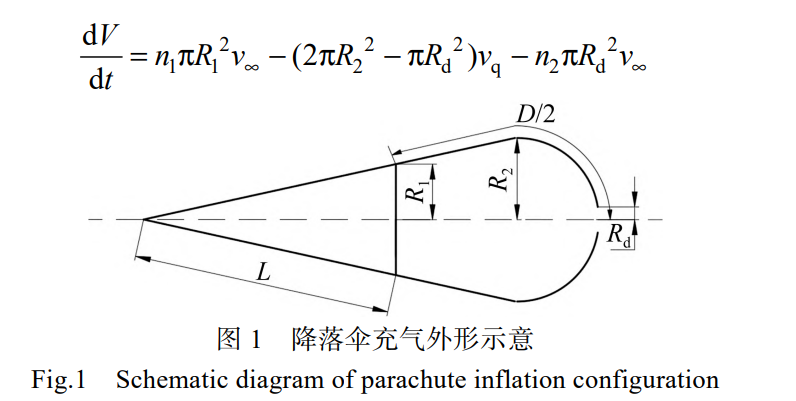
\includegraphics[width = 0.8\linewidth]{image/015.png}
\end{figure}

In the equation, \(V\) represents the internal volume of the canopy, \(t\) is the time, \(v_\infty \) is the incoming gas 
velocity, \(R_1\) is the radius of the lower edge of the inflated canopy, \(R_2\) is the radius of the upper hemisphere 
of the inflated canopy, \(R_d\) is the radius of the canopy top hole, which can also represent the air permeability 
of the canopy's top structure, \(v_q\) is the gas velocity exiting the canopy, representing the air permeability of 
the canopy fabric, \(n_1\) and \(n_2\) are correction factors that can be used to adjust the parameters in the formula 
as needed, \(D\) is the nominal diameter of the parachute, and \(L\) is the length of the parachute lines.

From the equation, it is evident that when there is \(dV/dt > 0\), it indicates that the canopy continues to inflate. 
Conversely, when \(dV/dt < 0\), it leads to parachute closing. The critical opening speed \(V_k\) is the value of \(v_\infty \) 
when \(dV/dt = 0\):

\begin{figure}[!hbtp]
    \centering 
    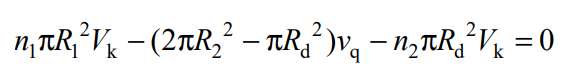
\includegraphics[width = 0.8\linewidth]{image/016.png}
\end{figure}

Therefore, the critical opening speed of the parachute is influenced by both parachute 
design parameters and atmospheric environmental parameters. In this context, we will not 
consider the impact of parachute design parameters, assuming constant parachute line length, 
geometric shape of the canopy, and canopy size. We will focus solely on the effect of atmospheric 
density on the critical opening speed.

Atmospheric density affects the effective air permeability of the fabric, where the effective air permeability \(W_y\) is given by:

\begin{figure}[!hbtp]
    \centering 
    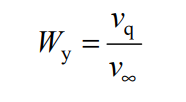
\includegraphics[width = 0.2\linewidth]{image/017.png}
\end{figure}

\newpage
Obtaining the effective air permeability of the fabric:

\begin{figure}[!hbtp]
    \centering 
    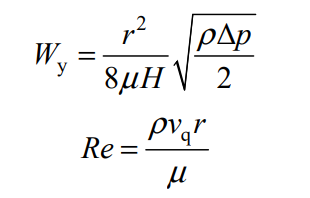
\includegraphics[width = 0.2\linewidth]{image/018.png}
\end{figure}

In the equation, \(r\) represents the radius of small holes in the fabric, \(\mu\) is the air viscosity coefficient, \(H\) is the fabric thickness, 
and \(Re\) is the Reynolds number. From the equation, it is evident that as atmospheric density increases, the Reynolds number increases, resulting in a greater 
effective air permeability of the fabric. The effective air permeability of the fabric is directly proportional to atmospheric density, and the critical opening 
speed is inversely proportional to the effective air permeability of the fabric (as indicated in a reference paper). Therefore, we can deduce that the critical 
opening speed is inversely proportional to atmospheric density.

Referring to a paper\cite{Sui}, we can derive the relationship between the critical opening speed and density as follows:

\[ \frac{V_k^2}{gD_0} = 2.74 \times 10^4 \left(\frac{\gamma_{avg}}{\rho D_0}\right)^{1.87} \]

Where \(\gamma\) is the crown density of the parachute, and \(D_0\) is the diameter of the parachute.

Through calculation, we can determine the critical speed for parachute deployment and thus constrain the jumping altitude.

\begin{figure}[!hbtp]
    \centering 
    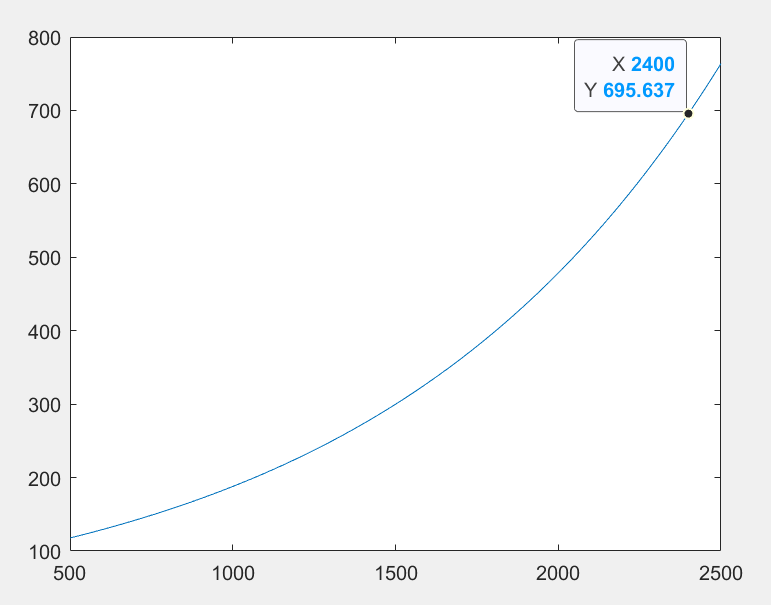
\includegraphics[width = 0.4\linewidth]{image/019.png}
    \caption{Critical speed for parachute deployment at different altitudes}
\end{figure}

Because the higher the opening altitude, the greater the speed that can be tolerated, we choose a height of 2400 meters as the opening altitude, 
and this is also the current world record for the opening altitude of a space diving.
The critical speed at this point is as follows:
\begin{figure}[!hbtp]
    \centering 
    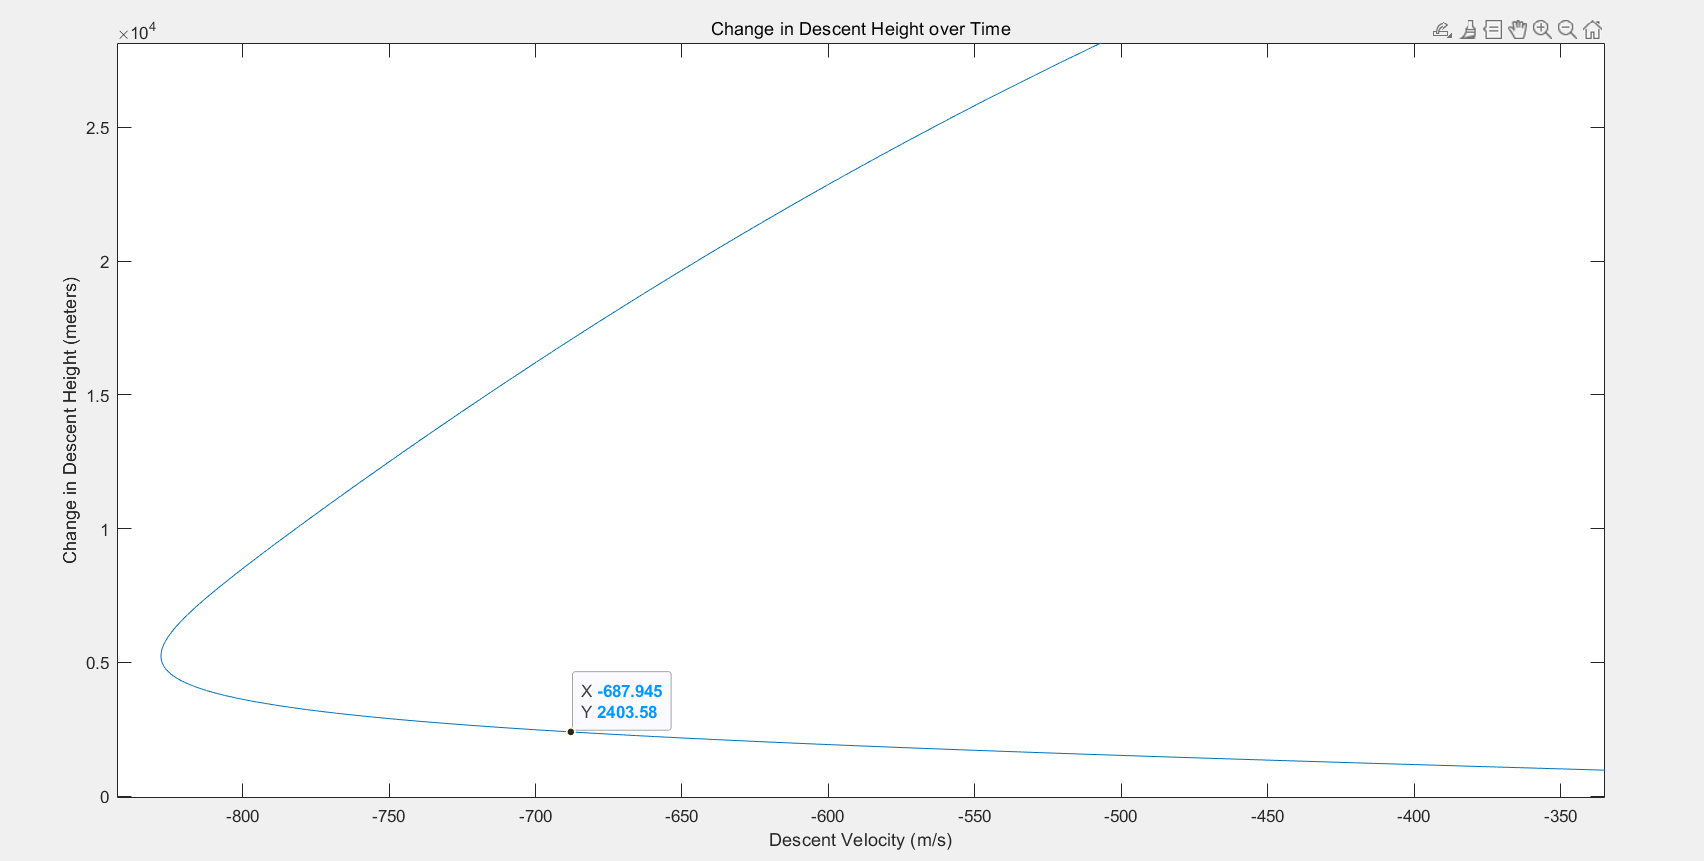
\includegraphics[width = 0.4\linewidth]{image/020.png}
    \caption{Critical speed for parachute deployment at 2400 m}
\end{figure}

Based on this constraint, assuming a parachute deployment at an altitude of 2400 meters, 
we need to jump from a height of \textbf{44110 meters}.

\subsection{Detailed analysis of parachute deployment process}

Given the significant threat to human life posed by the immense acceleration generated at the moment 
of parachute deployment, it is imperative to conduct a detailed analysis of this dynamic process. 
The parachute deployment process is highly intricate. 

At the same time, to enhance the safety of many parachutes, they require inflation before use. Inflating and expanding 
a parachute by introducing gas (typically air) ensures that it functions properly, slows down the 
descent, and makes the landing safer and more controllable. This process helps ensure that the 
parachute deploys rapidly when needed, providing the necessary air resistance to achieve a moderate 
descent rate, allowing the parachutist or cargo to land safely on the ground or in the target area.

In the following analysis, we neglect the influence of the following factors: the parachute's 
structure, its material properties, fluid flow instabilities, the aerodynamic effects of the parachute on 
the surrounding airflow, and the impact of crosswinds on parachute inflation.

\subsubsection{Three stages of parachute deployment}
Given the critical importance of safety, all the following analyses will 
take into account the scenario involving this inflatable parachute. 

We assume that the parachute is a single-stage choke. 
("Single-stage choke" is an engineering term used in the context of throttling or compression 
devices, typically within pipelines, piping systems, or other fluid transmission equipment. 
It refers to a system that employs only one valve or device to regulate or control the flow rate 
or pressure of the fluid.)

The inflation phase of the parachute can be divided into three stages:

\begin{itemize}
    \item \textbf{Stage One} ($t_{m1}$): The parachute begins to inflate, 
    and the canopy takes on a squid-like shape. 
    During this process, the drag area is linear with time.
    \item \textbf{Stage Two} ($t_{m2}$): The drag area remains constant at a value denoted as $A_{sk}$.
    \item \textbf{Stage Three} ($t_{m3}$): From the end of inflation until the canopy is fully extended, 
    the drag area remains at another constant value denoted as $A_p$. 
    In this stage, the drag area is a function of time to the power of $n$.
\end{itemize}

Here are the expressions for $A$ in each of the three stages\cite{jia2023parachute}:
\[
A = 
\begin{cases}
    \frac{A_{sk}}{t_{m1}}t, &  0 \leqslant t \leqslant t_{m1}\\
    A_{sk}, & t_{m1} < t \leqslant t_y\\
    A_{sk} + \left(A_p - A_{sk}\right)\left(\frac{t - t_y}{t_{m3}}\right)^n, & t_y < t \leqslant t_y + t_{m3}
\end{cases}
\]

Where:
\begin{itemize}
    \item $A$ represents the drag area.
    \item $n$ is the inflation parameter, typically ranging between 2 and 3.
    \item $t_y$ equals $t_{m1}+t_{m2}$.
\end{itemize}

From the calculations, it can be determined that the drag area $A$
during the first stage has a linear relationship with time: 
\[t_{m1} = \frac{\lambda_{m1}A_{sk}^{0.5}}{v_0}\]

Where:
\begin{itemize}
    \item $\lambda_{m1}$ is a certain constant.
    \item $v_0$ refers to the system's velocity relative to the ground at the moment when the parachute is deployed.
\end{itemize}

During the second stage, the drag area remains constant and there is no 
need to determine a relationship between the drag area and time.

In the third stage, the relationship between the drag area $A$ and time $t_{m3}$ is as follows:
\[t_{m3} = \frac{\lambda_{m3}\left(A_p^{0.5}-A_{sk}^{0.5}\right)}{v_1}\]

Where:
\begin{itemize}
    \item $\lambda_{m3}$ is a certain constant.
    \item $v_1$ refers to the velocity of the parachute and payload combination when the choke is fully closed.
\end{itemize}

\subsubsection{The impact of inertial resistance}
When an object experiences non-uniform motion in an ideal fluid, it encounters inertial resistance. 
Expressing inertial resistance in terms of momentum gives the impression of adding the mass of the 
fluid disturbed by the object, which is referred to as added mass.

Added mass, or virtual mass is the inertia added to a system because an accelerating or decelerating 
body must move (or deflect) some volume of surrounding fluid as it moves through it\cite{enwiki:1168352876}.

According to the drag area calculation method, the added mass of a parachute at a certain moment 
can be determined by the drag area, and the formula is as follows\cite{jia2023parachute}:
\[m_f = k_f \rho A^{1.5}\]

Where:
\begin{itemize}
    \item $k_f$ is the reference coefficient for added mass based on the drag area, which is typically determined experimentally.
    \item $\rho$ represents air density.
\end{itemize}

By considering the effect of inertial resistance, we can derive the 
rate of change of added mass with respect to time $\dot{m_f}$
during the inflation and deployment of the parachute as follows\cite{jia2023parachute}:
\[
\dot{m_f} = 
\begin{cases}
    1.5k_f\rho \left(\frac{A_{sk}}{t_{m1}}t\right)^{0.5}\frac{A_{sk}}{t_{m1}}, &  0 \leqslant t \leqslant t_{m1}\\
    0, & t_{m1} < t \leqslant t_y\\
    1.5k_f\rho \left[A_{sk}+(A_p-A_{sk})\left(\frac{t - t_y}{t_{m3}}\right)^n\right]^{0.5} \cdot n(A_p - A_{sk})\frac{(t-t_y)^{n-1}}{(t_{m3})^n}, & t_y < t \leqslant t_y + t_{m3}
\end{cases}
\]

\subsubsection{Safety analysis}

In the \textit{4.1 model}, we can observe that the most dangerous aspect for the human body during the entire 
parachute deployment process is excessive acceleration. Excessive acceleration not only causes trauma 
to the human body but can also lead to parachute line breakage. This issue can be quantified by 
calculating the opening load. The opening load comprises inertial forces, parachute fabric resistance, 
the reaction forces resulting from changes in added mass, and the gravitational force acting on the 
parachute.

To simplify the model, the following assumptions are made:
\begin{enumerate}
    \item Stretching of the parachute-payload combination is not considered.
    \item Lift forces on the parachute-payload combination are not considered.
    \item The analysis is conducted in a two-dimensional plane.
    \item The parachute-payload combination is treated as two point masses, with the mass concentrated at the 
    respective centers of mass for the payload and parachute. During the inflation phase, 
    the center of mass of the parachute remains fixed relative to the bottom edge.
    \item The axis of the parachute-payload combination remains straight during the inflation phase.
\end{enumerate}

\begin{minipage}{0.6\linewidth}
    The formula for the opening load can be derived\cite{gao2018achievements}: 
    \[ f_k = (m_p + m_f )\frac{dv}{dt} - \frac{1}{2}\rho v^2A + v\frac{dm_f}{dt} + m_p g \]
    And $\frac{dv}{dt}$ can be derived:
    \[ \dot{v} = -\frac{m_h}{m_p}g - \frac{1}{2}\rho v^2\frac{A_h + A}{m_h + m_p + m_f} - \frac{v}{m_h + m_p + m_f}\frac{dm_f}{dt}\]
    Where:
    \begin{itemize}
        \item $m_p$ is parachute mass and  $m_h$ is human mass. $m = m_p + m_h$.
        \item $A_h$ is the reference area of the parachutist and $A$ is the drag area of parachute. 
        \item $\rho $ is air density.
    \end{itemize}

\end{minipage}
\hfill
\begin{minipage}{0.3\linewidth}
    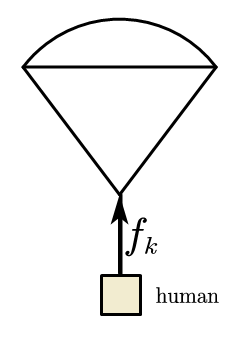
\includegraphics[width = \linewidth]{image/006.png}
    \captionof{figure}{Parachute diagram}
\end{minipage}

\vspace{12pt}
However, after the calculation, we have found that below a height of 44110 meters, 
the maximum acceleration does not exceed 20 times the gravitational 
acceleration, making it safe for a person.

\section{Conclusion}
In pursuit of determining the uppermost altitude achievable for a skydiving endeavor and assessing pertinent safety 
considerations inherent to the activity, this investigation has undertaken a comprehensive theoretical analysis of the 
discipline. We have employed two distinct idealized models: the first positing a uniform air density throughout the 
descent and the second recognizing the influence of altitude on atmospheric density. These models served as the foundation 
for scrutinizing the critical moment of parachute deployment, encompassing parachute tension and the pivotal critical opening speed.

Our inquiry has yielded the following discernments:

\begin{enumerate}
    \item In the inaugural model, neglecting the variances in air density concomitant with changing altitudes, 
    we observed that an individual embarking on a descent from a significant elevation (approximately 50 kilometers 
    above terrestrial ground) and initiating parachute deployment experiences a prodigious tension force, resulting 
    in an acceleration approximating 1000 m/s². This acceleration vastly surpasses the threshold of human physiological 
    tolerance, thus necessitating an intricate scrutiny of the circumstances attending the moment of parachute opening.

    \item In the second model, accounting for the impact of altitude on air density, we have established an altitude-air 
    density relationship, accommodating variations in atmospheric conditions. Owing to the constraints imposed by human 
    physiological limits, our analysis deduces a maximum skydiving altitude of 57,800 meters. Nevertheless, due to the precipitous descent 
    velocity, the safety of the descending individual is compromised, compelling the imperative for subsequent model refinements to ensure 
    their welfare.

    \item Emerging from the first model, it has come to our attention that the instant of parachute deployment holds paramount importance. 
    Through a meticulous dissection of the parachute deployment phase, along with rigorous computations of the load exerted during the 
    inflation stage, we ascertained that the actual maximum acceleration borne by the parachutist at the point of canopy deployment amounts 
    to 20g, well within the scope of tolerable physiological limits.

    \item To ascertain the reliable deployment of the parachute, the critical opening speed exhibits a positive correlation with altitude. 
    A rigorous evaluation entailing the manipulation of altitude values in conjunction with a comparative analysis relative to the critical 
    opening speed reveals a maximal skydiving altitude of 44,110 meters.
\end{enumerate}

In summation, cognizant of the multifarious factors involving dynamic air density, the consequential critical opening speed, 
and the exigencies of human physiological tolerance, our investigation culminates in the determination of the ultimate skydiving 
altitude attainable, set at 44,110 meters. However, in light of the existing records, including the zenith of world skydiving, 
registered at a maximum speed of 373 m/s, the model alludes to the prospect of enhanced refinement and further in-depth inquiry.


\section{Appendix}


\subsection{FirstBeforeChute.m}
The purpose of this code is to calculate the dynamic state before opening the parachute 
in the \textit{4.1 model} and generate corresponding graphs.
\begin{lstlisting}
    % Initialize parameters
    G = 6.67430e-11;   % Gravitational constant (m^3/kg/s^2)
    M = 5.972e24;      % Earth mass (kg)
    rho = 1.225;       % Air density (kg/m^3)
    c_h = 0.47;        % Air resistance coefficient for a person
    A_h = 1;           % Reference area for a person (m^2)
    m = 190;           % Person's mass (kg)

    % Set initial conditions
    r0 = 6421000; % Initial height (in meters)
    v0 = 0;    % Initial velocity is zero

    % Solve the differential equation
    tspan = [0, 500]; % Time interval
    t = linspace(tspan(1), tspan(2), 10000);
    f = @(t, y) [y(2); -G*M / y(1)^2 + 0.5 * c_h * rho * A_h / m * y(2)^2];
    [t, y] = ode45(f, t, [r0, v0]);

    descent_height_change = -y(1, 1) + y(:, 1);

    % Plot descent height and velocity curves
    figure;
    subplot(2, 1, 1);
    plot(t, descent_height_change); % Change in descent height as a function of time
    xlabel('Time (seconds)');
    ylabel('Change in Descent Height (meters)');
    title('Change in Descent Height over Time');

    subplot(2, 1, 2);
    plot(t, y(:, 2)); % Descent velocity as a function of time
    xlabel('Time (seconds)');
    ylabel('Descent Velocity (m/s)');
    title('Change in Descent Velocity over Time');
\end{lstlisting}



\subsection{FirstAfterChute.m}
The purpose of this code is to calculate the dynamic state after opening the parachute 
in the \textit{4.1 model} and generate corresponding graphs.
\begin{lstlisting}
    % Initialize parameters
    G = 6.67430e-11;   % Gravitational constant (m^3/kg/s^2)
    M = 5.972e24;      % Earth mass (kg)
    rho = 1.225;       % Air density (kg/m^3)
    c_p = 0.8;         % Air resistance coefficient for a person
    A_p = 70;          % Reference area for a person (m^2)
    m = 190;           % Person's mass (kg)

    % Set initial conditions
    r0 = 6372000; % Initial height (in meters)
    v0 = -80;    

    % Solve the differential equation
    tspan = [0, 50]; % Time interval
    t = linspace(tspan(1), tspan(2), 10000);
    f = @(t, y) [y(2); -G*M / y(1)^2 + 0.5 * c_p * rho * A_p / m * y(2)^2];
    [t, y] = ode45(f, t, [r0, v0]);

    descent_height_change = -y(1, 1) + y(:, 1);

    % Plot descent height and velocity curves
    figure;
    subplot(2, 1, 1);
    plot(t, descent_height_change); % Change in descent height as a function of time
    xlabel('Time (seconds)');
    ylabel('Change in Descent Height (meters)');
    title('Change in Descent Height over Time');

    subplot(2, 1, 2);
    plot(t, y(:, 2)); % Descent velocity as a function of time
    xlabel('Time (seconds)');
    ylabel('Descent Velocity (m/s)');
    title('Change in Descent Velocity over Time');

    % Calculate acceleration
    acceleration = diff(y(:, 2))./diff(t); % Calculate acceleration from velocity changes

    % Adjust the time interval to match the acceleration data
    t_acceleration = t(1:end-1);

    % Plot the relationship between acceleration and time
    figure;
    plot(t_acceleration, acceleration);
    xlabel('Time (seconds)');
    ylabel('Acceleration (m/s^2)');
    title('Change in Acceleration over Time');
\end{lstlisting}



\subsection{DensityVariation.m}
The purpose of this code is to calculate the relationship between air 
pressure and altitude in \textit{4.2 model} and then simplify 
it by fitting it into a function that is easier to work with in calculations.
\begin{lstlisting}
    % Define constants
    g = 9.80665;  % Acceleration due to gravity (m/s^2)
    M_a = 0.0289644;  % Mean molar mass of air (kg/mol)
    R_star = 8.31432;  % Universal gas constant (J/(molK))
    T0 = 288.15;  % Standard temperature at sea level (K)
    rho0 = 1.225;  % Standard air density at sea level (kg/m^3)

    % Define parameters
    height = 0:200:80000;  % Height range from 0 to 80000 meters with 200-meter intervals

    % Initialize air density vector
    rho = zeros(size(height));

    % Calculate air density
    for i = 1:length(height)
        h = height(i);
        
        % Determine the current atmospheric layer (based on the provided table)
        if h >= 0 && h < 11000
            Tb = T0 - 0.00649 * h;
            Lb = 0.00649;
            rho(i) = rho0 * ((Tb - (h - 0) * Lb) / Tb) ^ ((g * M_a) / (R_star * Lb) - 1);
        elseif h >= 11000 && h < 20000
            Tb = 216.65;
            Lb = 0;
            rhob = 0.36391;
            rho(i) = rhob * exp(-(g * M_a * (h - 11000) / (R_star * Tb)));
        elseif h >= 25000 && h < 32000
            Tb = 216.65;
            Lb = -0.001;
            rhob = 0.08803;
            rho(i) = rhob * ((Tb - (h - 25000) * Lb) / Tb) ^ ((g * M_a) / (R_star * Lb) - 1);
        elseif h >= 32000 && h < 47000
            Tb = 228.65 + 0.0028 * (h - 32000);
            Lb = -0.0028;
            rhob = 0.01322;
            rho(i) = rhob * ((Tb - (h - 32000) * Lb) / Tb) ^ ((g * M_a) / (R_star * Lb) - 1);
        elseif h >= 47000 && h < 51000
            Tb = 270.65;
            Lb = 0;
            rhob = 0.00143;
            rho(i) = rhob * exp(-(g * M_a * (h - 47000) / (R_star * Tb)));
        elseif h >= 51000 && h < 71000
            Tb = 270.65 - 0.0028 * (h - 51000);
            Lb = 0.0028;
            rhob = 0.00086;
            rho(i) = rhob * ((Tb - (h - 51000) * Lb) / Tb) ^ ((g * M_a) / (R_star * Lb) - 1);
        else
            Tb = 214.65 - 0.002 * (h - 71000);
            Lb = 0.002;
            rhob = 0.000064;
            rho(i) = rhob * ((Tb - (h - 71000) * Lb) / Tb) ^ ((g * M_a) / (R_star * Lb) - 1);
        end
    end

    % Plot the air density vs. height
    plot(height, rho);
    title('Air Density vs. Altitude');
    xlabel('Altitude (meters)');
    ylabel('Air Density (kg/m^3)');
    grid on;

    % Check and remove NaN values from the data
    valid_indices = ~isnan(rho);
    height_data = height(valid_indices);
    density_data = rho(valid_indices);

    % Define the exponential fit function
    expFitFunc = @(params, x) params(1) * exp(params(2) * x);

    % Initial guess for the parameters (a and b)
    initial_params = [1, -0.0001];

    % Perform the exponential fit using lsqcurvefit
    params = lsqcurvefit(expFitFunc, initial_params, height_data, density_data);

    % Extract the fitted parameters
    a = params(1);
    b = params(2);

    % Generate fitted data
    fit_density = expFitFunc(params, height_data);

    % Extract key data points
    keyPointsHeight = 0:1000:5000;  % Extract key data points for visualization
    keyPointsDensity = expFitFunc(params, keyPointsHeight);

    % Plot the exponential fit result
    figure;
    plot(height_data, density_data, 'o', 'DisplayName', 'Original Data');
    hold on;
    plot(height_data, fit_density, 'r', 'DisplayName', 'Exponential Fit');
    plot(keyPointsHeight, keyPointsDensity, 'bs', 'DisplayName', 'Key Points');
    legend;

    % Display the fitted equation on the plot
    equation = sprintf('Fitted Equation: y = %.4f * exp(%.4f * x)', a, b);
    text(10000, 0.01, equation, 'FontSize', 12);

    title('Fitting an Exponential Function to Data with Key Points');
    xlabel('Height (meters)');
    ylabel('Air Density (kg/m^3)');
    grid on;
\end{lstlisting}



\subsection{SecondBeforeChute.m}
The purpose of this code is to study the motion equations affected by 
changes in atmospheric density in the \textit{4.2 model}.
\begin{lstlisting}
    % Initialize parameters
    G = 6.67430e-11;   % Gravitational constant (m^3/kg/s^2)
    M = 5.972e24;      % Earth mass (kg)
    r_0 = 6371000;     % Earth radius (m)
    c_h = 0.8;        % Air resistance coefficient for a person
    S_h = 1;           % Reference area for a person (m^2)
    m = 190;           % Person's mass (kg)
    rho = 0.01322;     % Air density (kg/m^3)

    % Set initial conditions
    r0 = 6428800; % Initial height (in meters)
    v0 = 0;       % Initial velocity is zero

    % Time settings
    t_start = 0;          % Initial time
    t_end = 120;          % End time (adjust as needed)
    dt = 0.001;           % Time step

    % Create arrays to store the results
    t = t_start:dt:t_end;
    num_steps = length(t);
    r = zeros(1, num_steps);
    v = zeros(1, num_steps);
    a = zeros(1, num_steps);  % Array to store acceleration

    % Initialize the initial conditions
    r(1) = r0;
    v(1) = v0;

    % Solve the differential equation using Euler's method
    for i = 1:num_steps-1
        r_dot = v(i);
        
        % Check if the time is before 50 seconds
        if t(i) < 50
            v_dot = -G * M / r(i)^2 + 0.5 * (c_h * rho * S_h / m) * v(i)^2;
        else
            v_dot = -G * M / r(i)^2 + (0.64175 * exp(-0.001 * (r(i) - r_0)) * c_h * S_h) / m * v(i)^2;
        end
        
        a(i) = v_dot;  % Store acceleration
        
        r(i+1) = r(i) + r_dot * dt;
        v(i+1) = v(i) + v_dot * dt;
    end

    % Plot descent height, velocity, and acceleration curves
    figure;
    subplot(3, 1, 1);
    plot(t, r - r0); % Change in descent height as a function of time
    xlabel('Time (seconds)');
    ylabel('Change in Descent Height (meters)');
    title('Change in Descent Height over Time');

    subplot(3, 1, 2);
    plot(t, v); % Descent velocity as a function of time
    xlabel('Time (seconds)');
    ylabel('Descent Velocity (m/s)');
    title('Change in Descent Velocity over Time');

    subplot(3, 1, 3);
    plot(t, a); % Acceleration as a function of time
    xlabel('Time (seconds)');
    ylabel('Acceleration (m/s^2)');
    title('Acceleration over Time');
\end{lstlisting}



\subsection{SecondMaxAcc.m}
The purpose of this code is to study the maximum 
acceleration when descending from various heights in the \textit{4.2 model}.
\begin{lstlisting}
    % Initialize parameters
    G = 6.67430e-11;   % Gravitational constant (m^3/kg/s^2)
    M = 5.972e24;      % Earth mass (kg)
    r_0 = 6371000;     % Earth radius (m)
    c_h = 0.8;        % Air resistance coefficient for a person
    S_h = 1;           % Reference area for a person (m^2)
    m = 190;           % Person's mass (kg)

    % Time settings
    t_start = 0;          % Initial time
    t_end = 300;          % End time (adjust as needed)
    dt = 0.001;           % Time step

    % Define the range of initial heights
    initial_heights = 6381000:100:6451000; % Adjust the step size as needed

    % Initialize arrays to store results
    max_accelerations = zeros(size(initial_heights));

    % Loop through different initial heights
    for i = 1:length(initial_heights)
        r0 = initial_heights(i); % Set the initial height
        
        % Initialize arrays to store velocity and acceleration
        velocities = zeros(1, ceil((t_end - t_start) / dt));
        accelerations = zeros(1, ceil((t_end - t_start) / dt));
        
        % Initial conditions
        r = r0;
        v = 0;
        
        % Time loop
        t = t_start;
        j = 1;
        while t < t_end
            % Calculate gravitational force
            F_gravity = -G * M * m / r^2;
            
            % Calculate air resistance force
            F_air_resistance = 0.64175 * exp(-0.001 * (r - r_0)) * c_h * S_h * v^2;
            
            % Calculate acceleration
            acceleration = (F_gravity + F_air_resistance) / m;
            
            % Update velocity and position using the Verlet method
            v = v + acceleration * dt;
            r = r + v * dt;
            
            % Store velocity and acceleration at this time step
            velocities(j) = v;
            accelerations(j) = acceleration;
            
            % Update time
            t = t + dt;
            j = j + 1;
        end
        
        % Find and store the maximum acceleration
        max_accelerations(i) = max(abs(accelerations));
    end

    % Plot the relationship between initial height and maximum acceleration
    figure;
    plot(initial_heights, max_accelerations, 'o-');
    xlabel('Initial Height (m)');
    ylabel('Maximum Acceleration (m/s^2)');
    title('Relationship between Initial Height and Maximum Acceleration');
    grid on;
\end{lstlisting}


\bibliographystyle{unsrt}
\bibliography{paper.bib}

\end{document}
